Дадлагын 21 хоногийн хугацаанд "Branch Admin" гэх дотоодын программ дээр Front-End болон Back-End хөгжүүлэлтийг хийсэн. Уг системийн товч тайлбарлавал дуудлагын төв болон хэрэглэгчид үйлчлэх төвд ажиллаж байгаа ажилтан боруулалт хийх болон хэрэглэгчид тулгарсан асуудалыг шийдвэрлэх процессыг хөнгөвчлөх зорилготой. Мөн борлуулалт хянах тайлан гаргах боломжтой систем юм.
\section{Хэрэглэгчийн шаардлага}

  \subsection{Хэрэглэгчид}
    \begin{itemize}
        \item Админ болон салбарын ажилтнууд орно.
    \end{itemize}

  \subsection{Функционал хэрэглэгчийн шаардлагууд}
    \begin{itemize}
        \item Хэрэглэгчийн бүртгэл хийх, шинэчлэх, устгах боломжтой байх.
        \item Систем нь хэрэглэгчийн мэдээллийг найдвартай хадгалж, аюулгүй байдлыг хангах ёстой.
        \item Үйлчлүүлэгчийн үйлчилгээний мэдээллийг хянах, шинэчлэх, засварлах боломжтой байх.
        \item Систем нь олон хэрэглэгчийн нэгэн зэрэг оролцох боломжыг дэмжих ёстой.
        \item Систем нь хэрэглэгчийн хүсэлт, гомдлыг хүлээн авч, шийдвэрлэх ажиллагааг дэмжих.
    \end{itemize}

  \subsection{Функционал бус шаардлага}
    \begin{itemize}
        \item Систем нь хурдан ачаалагдах, бага хүлээх хугацаатай байх ёстой.
        \item Хэрэглэгчийн интерфэйс энгийн, ойлгомжтой, хэрэглэгчдэд хялбар байх.
        \item Систем нь олон хэрэглэгчийн нэгэн зэрэг оролцох чадвартай байх.
        \item Системийн аюулгүй байдал өндөр байх ёстой, түүнд нэвтрэх эрхгүй хүн орох боломжгүй байх.
        \item Систем нь өргөжүүлэлт хийх боломжтой, шинэ хэрэглэгчид болон үйлчилгээг дэмжих чадвартай байх.
    \end{itemize}

\pagebreak

\section{Use Case диаграм}
\begin{figure}[h!]
	\centering
	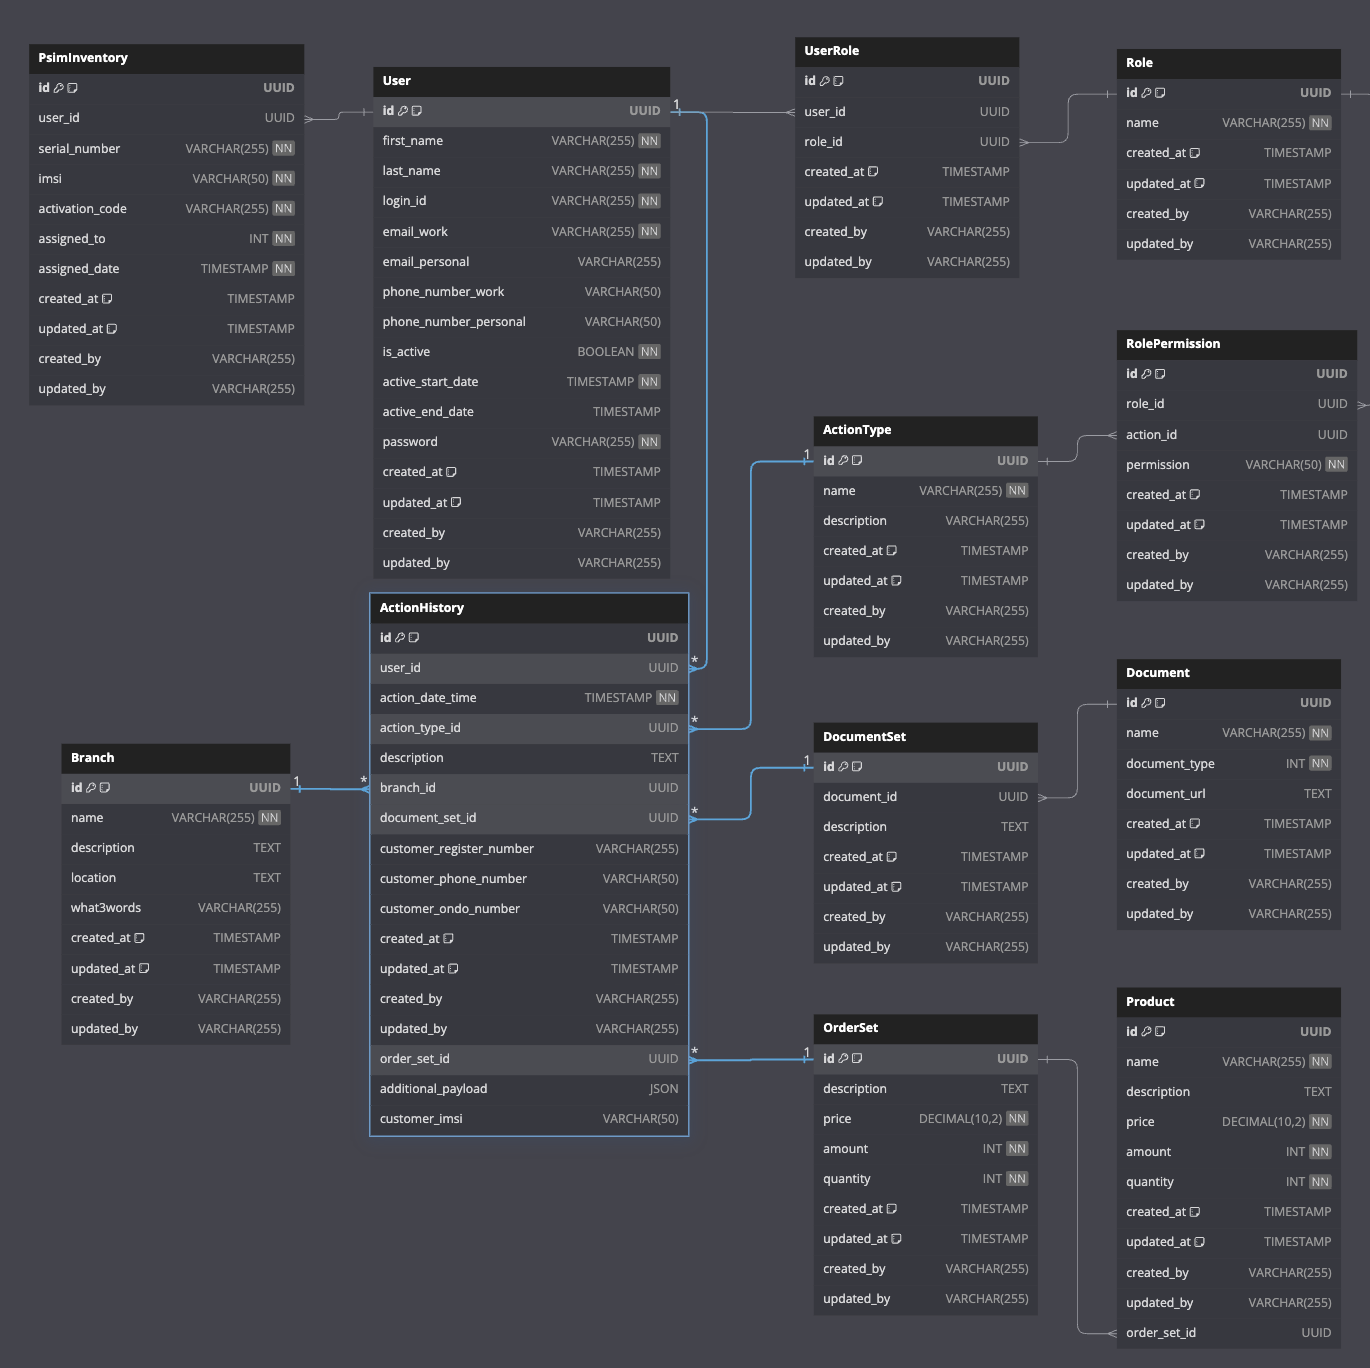
\includegraphics[width=15cm]{images/usecase-diagram.png}
	\caption{Use Case диаграм}
	\label{fig:usecase-image}
\end{figure}
\pagebreak

\section{Entity Relationship диаграм}
\begin{figure}[h!]
	\centering
	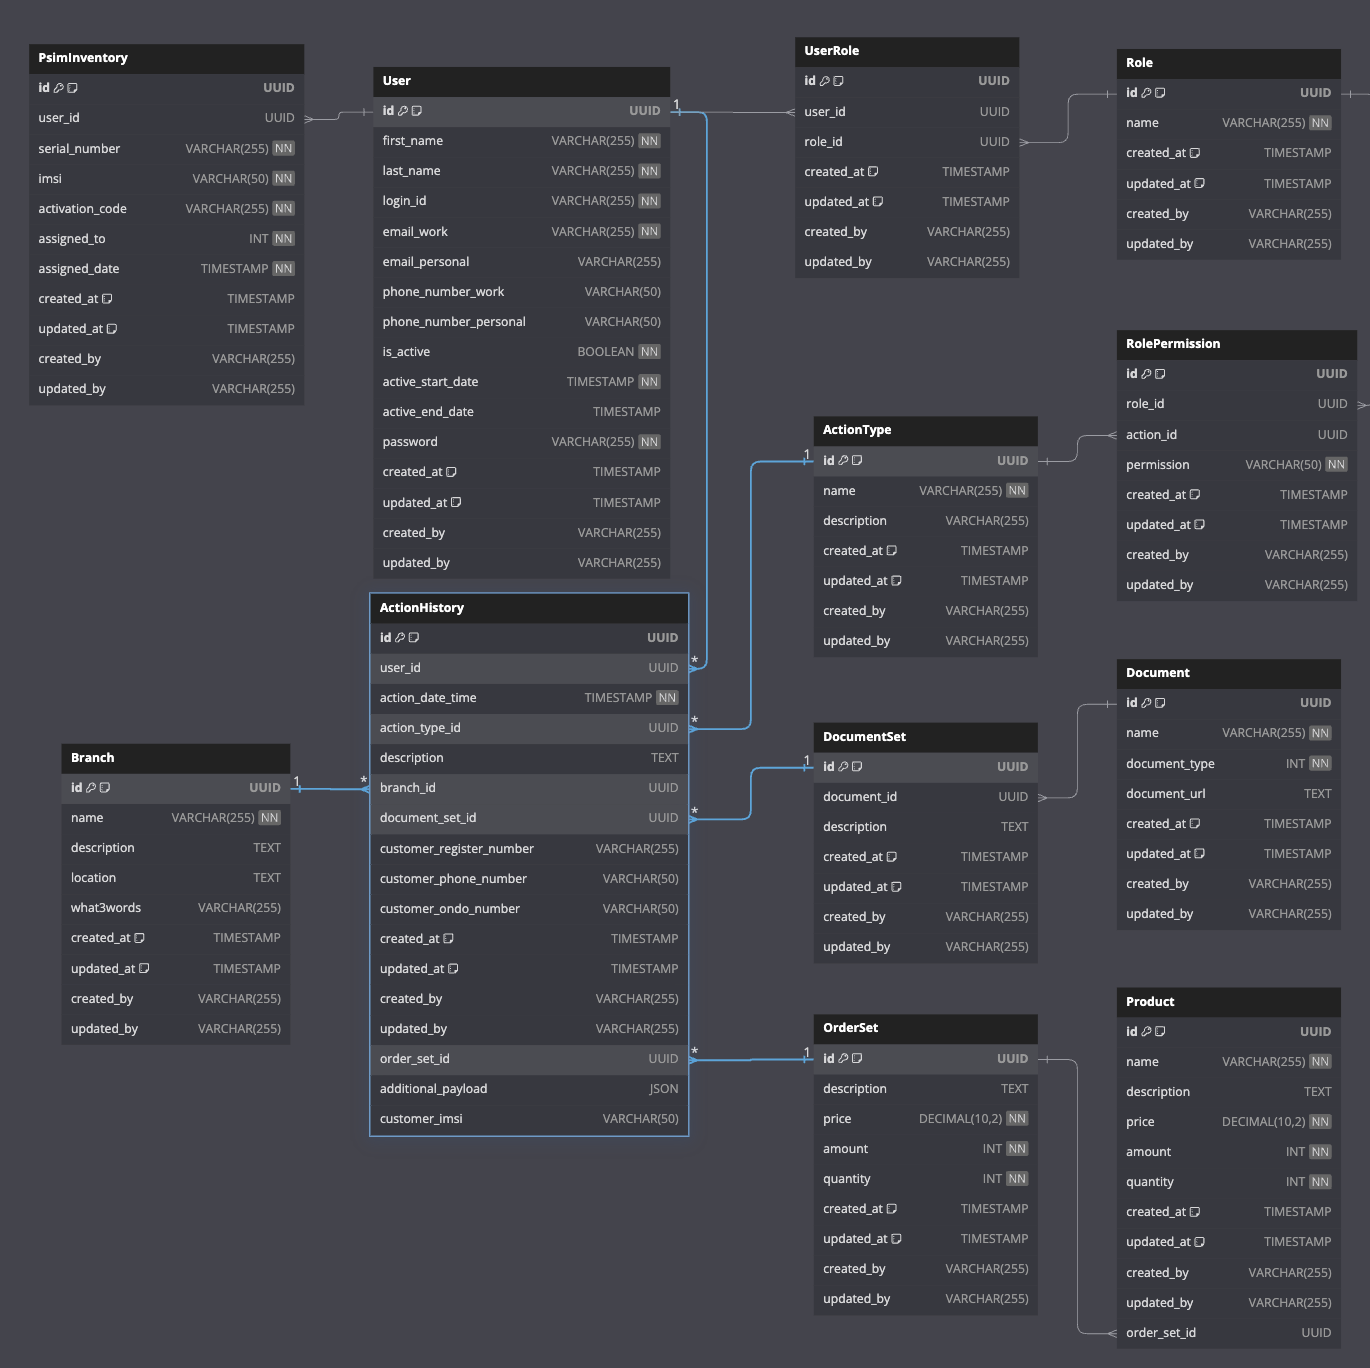
\includegraphics[width=15cm]{images/er-diagram.png}
	\caption{Entity Relationship диаграм}
	\label{fig:er-image}
\end{figure}